%% LyX 2.3.0 created this file.  For more info, see http://www.lyx.org/.
%% Do not edit unless you really know what you are doing.
\documentclass[UTF8]{ctexart}
\usepackage[T1]{fontenc}
\usepackage{geometry}
\geometry{verbose,tmargin=3cm,bmargin=3cm,lmargin=3cm}
\usepackage{calc}
\usepackage{amsmath}
\usepackage{amssymb}

\makeatletter
%%%%%%%%%%%%%%%%%%%%%%%%%%%%%% User specified LaTeX commands.
% 如果没有这一句命令,XeTeX会出错,原因参见
% http://bbs.ctex.org/viewthread.php?tid=60547
\DeclareRobustCommand\nobreakspace{\leavevmode\nobreak\ }
\usepackage{pgfplots}
\usepackage{pgf,tikz,pgfplots}
% \pgfplotsset{compat=1.15}
\usepackage{mathrsfs}
\usetikzlibrary{arrows,intersections}
\usepackage{tkz-euclide}
\usetkzobj{all} 

\providecommand{\abs}[1]{\left\lvert#1\right\rvert}
\providecommand{\norm}[1]{\lVert#1\rVert}
\providecommand{\paren}[1]{\left(#1\right)}
\newcommand{\Integers}{\mathbb{Z}}
\newcommand{\Naturals}{\mathbb{N}}
\newcommand{\Rationals}{\mathbb{Q}}
\newcommand{\Reals}{\mathbb{R}}
\newcommand{\Complexes}{\mathbb{C}}
\newcommand{\pNaturals}{\mathbb{N}_{+}}

\def\ue{\mathrm{e}}
\def\ud{\,\mathrm{d}}
\def\GF{\mathrm{GF}}
\def\ui{\mathrm{i}}
\def\Re{\mathrm{Re}}
\def\Im{\mathrm{Im}}
\def\Res{\mathrm{Res}}
\def\diag{\,\mathrm{diag}\,}

\makeatother

\begin{document}

\title{上海市高中数学竞赛试题}

\author{Larry Eppes}
\maketitle

\section{1980年上海市高中数学竞赛试题}

\subsection{一试}

\paragraph{1. }

已知$a>1$, $b>1$, 求证$\log_{a}ab+\log_{b}ab\ge4$.

这题比较简单, 首先想到恒等式$\log_{x}y=\frac{\log y}{\log x}$对于所有正实数$x,y$都成立,
所以

\[
LHS=\frac{\log ab}{\log a}+\frac{\log ab}{\log b}=\log ab\paren{\frac{1}{\log a}+\frac{1}{\log b}}
\]
另外恒等式$\log ab=\log a+\log b$对于所有的正实数$a,b$都成立. 另外, 因为$x>1$时$\log x>0$.
所以如果用均值不等式, 则有

\[
\frac{\log ab}{\log a}+\frac{\log ab}{\log b}=1+\frac{\log b}{\log a}+\frac{\log a}{\log b}+1\ge1+2\sqrt{\frac{\log b}{\log a}\cdot\frac{\log a}{\log b}}+1=4
\]
如果考虑使用Cauchy不等式, 则有

\[
\log ab\paren{\frac{1}{\log a}+\frac{1}{\log b}}=\paren{\log a+\log b}\paren{\frac{1}{\log a}+\frac{1}{\log b}}\ge\paren{1+1}^{2}.
\]


\paragraph{2. }

设$x_{1}$, $x_{2}$是方程$x^{2}-x+1=0$的两个根, 求$x_{1}^{1980}+\paren{\frac{1}{x_{2}}}^{1980}$的值.

次数真高, 但是因为有个倒数, 而且韦达定理说两根的积

\[
x_{1}x_{2}=1
\]
这样可以求出来$\frac{1}{x_{2}}=x_{1}$, 但代入最后的式子里还是次数太高, 变成了$2x_{1}^{1980}$.
但是这一不是不可求解的, 因为$x_{1}$是方程$x^{2}-x+1=0$的根, 所以$x_{1}^{2}=x_{1}-1$,
这样两边乘以$x_{1}^{n}$, 并记$X_{n}=x_{1}^{n}$就会出现$X_{n+2}=X_{n+1}-X_{n}$这刚好是一个递推公式,
而且可以计算出

\[
X_{0}=1,X_{1}=2x_{1},X_{2}=2x_{1}-1,X_{3}=-1,X_{4}=-2x_{1},X_{5}=-2x_{1}+1,X_{6}=1,X_{7}=2x_{1}
\]
这样一直算下来形成了一个周期, 也是太巧了, 可以看出$X_{k+6}=X_{k}$, 但是证明的话还是要用归纳法或者自然数的良序性.
所以只需要知道$1980=6\times330$便知$X_{1980}=X_{0}=1$, 注意$X_{n}=x_{1}^{n}$而要求的结果是$2x_{1}^{1980}$.

\paragraph{3. }

设$D$为$\triangle ABC$的边$BC$上的点, 连接$AD$得$\triangle ABD$和$\triangle ACD$如果这三个三角形相似,
问$\triangle ABC$是怎样的三角形? 为什么?

图形比较简单的问题, 可以入手的方向会比较简单, 考虑角度$\angle ADB$和$\angle ADC$, 它们是一对邻补角,
所以它们之中必然有一个至少是$90^{\circ}$. 

如果$\angle ADB=\angle ADC=90^{\circ}$, 那么按相似的点的顺序$A,B,D$对应$A,C,D$或者$C,A,D$,
而前面的相似三角形对应关系中有公共边$AD$, 可以考虑$AAS$或$ASA$证明出$\triangle ABD\cong\triangle ACD$,
这说明$\triangle ABC$是等腰三角形; 而后面的三角形的对应关系说明$90^{\circ}=\angle BAD+\angle ABD=\angle BAD+\angle CAD$,
这说明$\angle A$是$\triangle ABC$的直角顶点. 

如果$\angle ADB$和$\angle ADC$之一大于$90^{\circ}$, 则另一个小于$90^{\circ}$.
比如$\angle ADB>90^{\circ}$, $\angle ADC<90^{\circ}$. 因为$\angle ADB$作为$\triangle ACD$的外角,
所以所以$\angle ADB$比$\triangle ACD$的任何内角都大, 这时候的$\triangle ADB$和$\triangle ADC$不可能相似.

\paragraph{4. }

已知$\triangle ABC$的边$BC$上有两点$D,E$, 且$BD=CE$. 求证: $AB+AC>AD+AE$.

条件$BD=CE$并不能确定$B,C,D,E$四个点的位置顺序是$B,D,E,C$还是$B,E,D,C$, 但是如果$D=E$,
问题就变成了$AB+AC>2AD=2AE$. 这暗示我们直接延长$AD$构造一个平行四边形就能证明了. 如果$D\ne E$,
也可以构造平行四边形, 如下图所示的那样. 

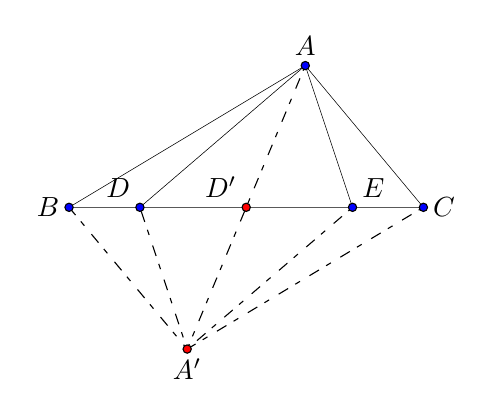
\begin{tikzpicture}[scale=0.3] 
\coordinate[label=90:$A$] (A) at(10,6);
\coordinate[label=180:$B$](B) at(0,0);
\coordinate[label=0:$C$](C) at(15,0);
\coordinate[label=135:$D$](D) at(3,0);
\coordinate[label=45:$E$](E) at(12,0);
\coordinate[label=135:$D'$](Dp) at(7.5,0);
\coordinate[label=270:$A'$](Ap) at(5,-6);
\draw [very thin] (A) -- (B) -- (C) -- (A);
\draw [very thin] (D) -- (A) -- (E);
\draw [dash pattern=on 2pt off 3pt on 4pt off 4pt] (A) -- (Ap) -- (B);
\draw [dash pattern=on 2pt off 3pt on 4pt off 4pt] (C) -- (Ap) -- (D);
\draw [dash pattern=on 2pt off 3pt on 4pt off 4pt] (E) -- (Ap);
\draw [fill=blue] (A) circle (5pt); 
\draw [fill=blue] (B) circle (5pt); 
\draw [fill=blue] (C) circle (5pt); 
\draw [fill=red] (Ap) circle (5pt);
\draw [fill=blue] (D) circle (5pt); 
\draw [fill=blue] (E) circle (5pt); 
\draw [fill=red] (Dp) circle (5pt);
\end{tikzpicture}

其中$D'$是$BC$的中点, 延长$AD'$到$A'$使得$AD'=A'D'$, 连接其它几条边. 这样$AE=A'D$,
$AC=A'B$, 问题转化为$AB+BA'>AD+DA'$, 当$ABA'D$是一个凹四边形时, 便成为一个较旧的问题:

\noindent\fbox{\begin{minipage}[t]{1\columnwidth - 2\fboxsep - 2\fboxrule}%
凹四边形$ABCD$, 如果角$\angle D$大于$180^{\circ}$, 则$AB+AC>DB+DC$.%
\end{minipage}}

所以可以照搬问题的证明, 延长$AD$交$BA'$于一点$F$, 根据三角不等式就有

\[
AB+BA'=AB+BF+FA'\ge AF+FA'=AD+DF+FA'\ge AD+DA'
\]

另外对于不等式来说, 它刚好是两个三角形的两边之和, $AB+AC$是三角形$\triangle ABC$的两边的和, $AD+AE$是三角形$\triangle ADE$的两边的和.
也有考虑通过添项使不等式仍然成立, 比如$BD+AB+AC>AD+AE+CE$, 由三角不等式$BD+AB>AD$, 但是$AC<AE+CE$还是不能给出证明.
也有分类讨论来证明的, 分类依据是: 过$A$做$BC$的垂线$AH$, 如果$D,E$在点$H$的两侧, 问题是容易证明的,
如果$D,E$在$H$的同一侧, 可以考虑点$E$关于$H$的对称点$E'$, 这样$AE=AE'$, 但是如果$E'$在$H$和$C$之间,
问题可以同前面一样证明, 但如果$E'$在$BC$的延长线上, 证明将不会通过! 所以这些方法都是行不通的.

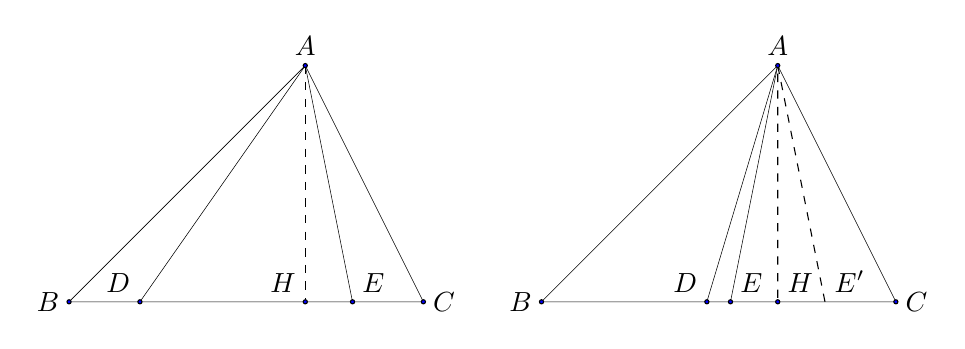
\begin{tikzpicture}[scale=0.3] 
\coordinate[label=90:$A$] (A) at(10,10);
\coordinate[label=180:$B$](B) at(0,0);
\coordinate[label=0:$C$](C) at(15,0);
\coordinate[label=135:$D$](D) at(3,0);
\coordinate[label=45:$E$](E) at(12,0);
\coordinate[label=135:$H$](H) at(10,0);
\draw [very thin] (A) -- (B) -- (C) -- (A); 
\draw [very thin] (A)-- (D); 
\draw [very thin] (A)-- (E);
\draw [dashed] (A) -- (H);
\draw [fill=blue] (A) circle (2.5pt); 
\draw [fill=blue] (B) circle (2.5pt); 
\draw [fill=blue] (C) circle (2.5pt); 
\draw [fill=blue] (H) circle (2.5pt);
\draw [fill=blue] (D) circle (2.5pt); 
\draw [fill=blue] (E) circle (2.5pt); 
\coordinate[label=90:$A$] (A2) at(30,10);
\coordinate[label=180:$B$](B2) at(20,0);
\coordinate[label=0:$C$](C2) at(35,0);
\coordinate[label=135:$D$](D2) at(27,0);
\coordinate[label=45:$E$](E2) at(28,0);
\coordinate[label=45:$H$](H2) at(30,0);
\coordinate[label=45:$E'$](Ep) at (32,0);
\draw [very thin] (A2) -- (B2) -- (C2) -- (A2); 
\draw [very thin] (A2)-- (D2); 
\draw [very thin] (A2)-- (E2);
\draw [dashed] (Ep)--(A2) -- (H2);
\draw [fill=blue] (A2) circle (2.5pt); 
\draw [fill=blue] (B2) circle (2.5pt); 
\draw [fill=blue] (C2) circle (2.5pt); 
\draw [fill=blue] (H2) circle (2.5pt);
\draw [fill=blue] (D2) circle (2.5pt); 
\draw [fill=blue] (E2) circle (2.5pt); 
\end{tikzpicture}

\paragraph{5. }

非零实数$a,b,c,x,y,z$满足条件$a^{2}+b^{2}+c^{2}=x^{2}+y^{2}+z^{2}=ax+by+cz$,
求证: $\frac{x}{a}=\frac{y}{b}=\frac{z}{c}$.

看到这个条件就想到了配平方, 计算

\[
0=a^{2}+b^{2}+c^{2}+x^{2}+y^{2}+z^{2}-2ax-2by-2cz=(a-x)^{2}+(b-y)^{2}+(c-z)^{2}
\]
所以$a=x$, $b=y$, $c=z$, 而在$a,b,c,x,y,z$是非零实数的时候$a,b,c$可以做分母.

\paragraph{6. }

$\triangle ABC$中最大角$A$是最小角$C$的$2$倍, 夹角$A$的两边$b=5$, $c=4$. 求第三边$a$和$\triangle ABC$的面积.

这题的条件是$\angle A=2\angle C$, 所以$\sin A=\sin2C=2\sin C\cos C$, 而$\cos C=\frac{a^{2}+b^{2}-c^{2}}{2ab}$,
正弦定理表明$\frac{\sin A}{\sin C}=\frac{a}{c}$. 代入$b=5$, $c=4$就会有

\[
a=2c\frac{a^{2}+b^{2}-c^{2}}{2ab}=4\cdot\frac{a^{2}+9}{5a}
\]
也就是$a^{2}=36$, $a=6$. 再用海伦公式$S=\sqrt{p(p-a)(p-b)(p-c)}$即可.

也可以建立角度的恒等式, 因为$b:c=5:4$, 由正弦定理有$\sin B:\sin C=5:4$, 而已知$\angle A=2\angle C$,
建立$\angle B,\angle C$的方程, 则$\pi=\angle B+3\angle C$, 所以$\sin B=\sin3C$,
所以$\sin3C:\sin C=5:4$, 再考虑三倍角公式有$\sin3C=3\sin C-4\sin^{3}C$, 所以$7/16=\sin^{2}C$,
再解出$\cos C$, 根据倍角公式$\sin2C=2\sin C\cos C$算出$\sin A$, 最后用面积公式$S=\frac{1}{2}bc\sin A$算出结果.

\paragraph{7. }

已知平面的斜线在此平面上的射影与该平面内过此斜线足的两直线构成等角, 求证: 斜线本身与上述两直线也构成等角.

可以用空间余弦定理

\[
\cos\alpha=\frac{\cos\delta-\cos\beta\cos\gamma}{\sin\beta\sin\gamma}
\]
来证明.

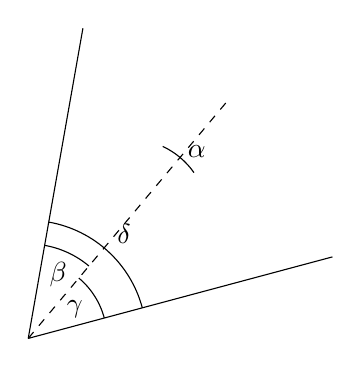
\begin{tikzpicture}
\coordinate (A) at (0,0);
\draw (A) -- ++(15:4cm);
\draw[dashed] (A) -- ++(50:4cm);
\draw (A) -- ++(80:4cm);
\draw (A) +(15:1cm) arc [start angle=15,end angle=50,radius=1cm];
\draw (A) +(50:1.2cm) arc [start angle=50,end angle=80,radius=1.2cm];
\draw (A) +(15:1.5cm) arc [start angle=15,end angle=80,radius=1.5cm];
\draw (A) +(50:3cm) arc[start angle=50,end angle=65,radius=1cm];
\draw (A) +(50:3cm) arc[start angle=50,end angle=35,radius=1cm];
\path (A) +(32.5:0.7cm) node {$\gamma$};
\path (A) +(65:0.9cm) node {$\beta$};
\path (A) +(47.5:1.8cm) node {$\delta$};
\path (A) +(48:3.2cm) node {$\alpha$};
\end{tikzpicture}

\paragraph{8. }

已知函数$y=\sin^{2}x+\cos x+\frac{1}{4}$, 问$x$取何值时, 函数$y$有极值.

看到$\cos x$是一次的, $\sin^{2}x=1-\cos^{2}x$, 所以$y=-\cos^{2}x+\cos x+\frac{5}{4}$,
而这与二次方程$y=-t^{2}+t+\frac{5}{4}$在$-1\le t\le1$时的极值问题相同, 注意$t$的范围.

\paragraph{9. }

设$P$点在双曲线$x^{2}-y^{2}=1$上运动, $P$处切线与圆$x^{2}+y^{2}=1$交于$A$和$B$,
求弦$AB$中点$Q$的轨迹方程.

直接解析法求解, 设$P$的坐标为$(x_{P},y_{P})$, 那么经过$P$的切线的方程是$x_{P}x-y_{P}y=1$.
解出$x_{P}x$并对方程$x^{2}+y^{2}=1$两边同时乘以$x_{P}^{2}$, 得到$(x_{P}^{2}+y_{P}^{2})y^{2}+2y_{P}y+1-x_{P}^{2}=0$,
用韦达定理算出$Q$的纵坐标$y_{Q}=-\frac{y_{P}}{x_{P}^{2}+y_{P}^{2}}$, 再代入$x_{P}x-y_{P}y=1$解出$x_{Q}=\frac{x_{P}}{x_{P}^{2}+y_{P}^{2}}$,
为了得到轨迹方程, 先计算$x_{Q}^{2}+y_{Q}^{2}$, 再计算$x_{Q}^{2}-y_{Q}^{2}$, 便得到轨迹方程$x^{2}-y^{2}=(x^{2}+y^{2})^{2}$,
但是\textbf{注意}在点$P$连续变化时$Q$的位置不能取到原点, 所以轨迹方程中应当去掉原点.

另一方法是用圆的性质, 垂直于弦的直径平分弦, 因为过$P$的切线$x_{P}x-y_{P}y=1$与圆$x^{2}+y^{2}=1$交于两点$A,B$,
而过$O$垂直于$AB$的直线过$AB$的中点$Q$, 这个直线的方程是$y_{P}x+x_{P}y=0$, 联立方程求解.

\subsection{二试}

\paragraph{1. }

已知$\triangle ABC$中, $\log\tan A+\log\tan C=2\log\tan B$, 求角$B$的范围.

首先根据定义域, $\tan A>0$, $\tan C>0$, $\tan B>0$, 所以$\triangle ABC$是锐角三角形.
但只这么说明还是不够因为广义的来说无穷大等于无穷大, 当等式两边有一个是无穷大, 则必有一个角是$90^{\circ}$, 而另两个角就只能是锐角,
不符合等式.

然后$\tan^{2}B=\tan A\tan C$, 如果考虑消元法, $\tan C=-\tan(A+B)=-\frac{\tan A+\tan B}{1-\tan A\tan B}$,
所以

\[
\tan^{2}A+(1-\tan^{2}B)\tan B\tan A+\tan^{2}B=0
\]
方程看成$\tan A$的二次函数恒有正根, 这一点通过两根的积是正的说明, 两个根同号, 并根据$\tan A=0$时上式左边是正的,
也就是对应的二次函数与$y$轴交于正半轴, 所以需要保证二次函数的对称轴是正的, 应该考虑为什么对称轴不能是$y$轴. 所以

\[
\tan B(1-\tan^{2}B)<0
\]
这说明$B>\frac{\pi}{4}$. 但这还没完, 因为对称轴为正不能保证二次函数有零点, 所以还要求判别式非负, 而这将说明

\[
\tan^{2}B(1-\tan^{2}B)^{2}-4\tan^{2}B\ge0
\]
所以$\tan B\ge\sqrt{3}$, 也就是$B\ge\frac{\pi}{3}$. 最后还要说明$\frac{\pi}{3}\le B<\frac{\pi}{2}$中的任何角$B$都是合情合理的,
对于$\frac{\pi}{3}$可以考虑正三角形, 而另一边在$B$的任何值都将导致前面的二次方程有个正解, 同时$\tan A$是方程的一个解,
而另一个解可以根据韦达定理$\tan A\cdot x_{2}=\tan^{2}B=\tan A\tan C$而求得, 也就是$\tan A$,
$\tan C$都是前面那个二次方程的根, 根据对乘轴的位置和判别式的正负性就可知道$\tan A$, $\tan C$是由$\tan B$决定的两个正值.

\paragraph{2. }

在单位正方体$ABCD-A'B'C'D'$中, 在一个面的对角线$AB'$上取$M$点使$AB'=3AM$, 在另一个面的对角线$BD$上取$N$点使$BD=3BN$.
求证: $MN$是$AB'$和$BD$的公垂线, 并求$MN$的长.

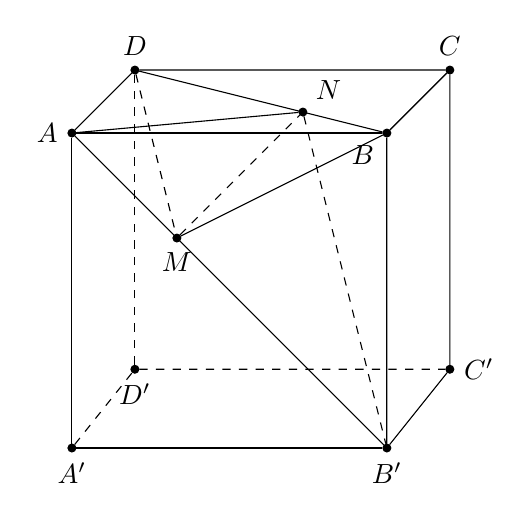
\begin{tikzpicture} 
\foreach \n/\x/\l/\p in{ 
1/{( 0  , 0)}/{$A'$}/below, 
2/{( 4, 0)}/{$B'$}/below, 
3/{( .8, 1)}/{$D'$}/below, 
4/{( 4.8, 1)}/{$C'$}/right, 
5/{( 0, 4)}/{$A$}/left, 
6/{( 4, 4)}/{$B$}/south west, 
7/{( 0.8, 4.8)}/{$D$}/above, 
8/{( 4.8, 4.8)}/{$C$}/above,
9/{( 4/3,8/3)}/{$M$}/below,
10/{(8.8/3,12.8/3)}/{$N$}/above right
} { 
       \node[inner sep=1pt,circle,draw,fill,label={\p:\l}] (\n) at \x {};    
} 
\draw (1) -- (2) -- (6) -- (5) -- (1); 
\draw (5) -- (6) -- (8) -- (7) -- (5); 
\draw (2) -- (4) -- (8) -- (6) -- (2); 
\draw[dashed] (1) -- (3) -- (4); 
\draw[dashed] (3) -- (7); 
\draw (10) -- (5) -- (2);
\draw (9) -- (6) -- (7);
\draw[dashed] (9) -- (10);
\draw[dashed] (7) -- (9);
\draw[dashed] (10) -- (2);
\end{tikzpicture}

在立体几何中有个方便的结论是

\noindent\fbox{\begin{minipage}[t]{1\columnwidth - 2\fboxsep - 2\fboxrule}%
如果$AB\perp CD$, 则$P_{ACBD}=AC^{2}-CB^{2}+BD^{2}-DA^{2}=0$.%
\end{minipage}}

此结论被称为勾股差, 在张景中院士的新概念几何里有更详细的说明, 而且这一结论在平面几何和立体几何中都是成立的. 用这个结论可以轻易解决本问题.

坐标法也是常见的方法, 计算过程比较机械.

\paragraph{3. }

抛物线与$Oy$轴相切于原点, 直线$x+y+1=0$是抛物线在顶点的切线, 求此抛物线的方程.

用坐标旋转公式, 坐标旋转公式的证明可以使用复数, 设原坐标为$(x,y)$, 新坐标为$(X,Y)$, 如果新坐标需要通过旧坐标绕原点$O$逆时针旋转$\theta$角来得到,
则有关系$X+Y\ui=(x+y\ui)\ue^{\ui\theta}$, 利用欧拉公式就有

\[
\begin{cases}
X=x\cos\theta-y\sin\theta\\
Y=x\sin\theta+y\cos\theta
\end{cases}
\]
所以先将要求的抛物线顺时针旋转$45^{\circ}$, 旋转后的抛物线将与$X=\frac{\sqrt{2}}{2}$相切,
这个值通过将$\theta=-\frac{\pi}{4}$代入上式便可得到. 所以这个抛物线的方程可以设为$X=a\paren{Y-b}^{2}+\frac{\sqrt{2}}{2}$.
因为旋转是绕原点进行, 原抛物线过原点, 所以旋转后仍然过原点, 所以$ab^{2}+\frac{\sqrt{2}}{2}=0$.
另外$Oy$轴绕原点顺时针旋转$45^{\circ}$得到直线$y=x$, 它与新抛物线相切, 代入抛物线方程也就是$a\paren{Y-b}^{2}-(X-b)-b+\frac{\sqrt{2}}{2}=a\paren{Y-b}^{2}-(Y-b)-b+\frac{\sqrt{2}}{2}=0$有重根,
所以$\Delta=1-4a\paren{-b+\frac{\sqrt{2}}{2}}=0$, 这样去解$a,b$, 再将抛物线旋转回去就好了.

\paragraph{4. }

证明: 
\[
F=\sqrt{2}+\sqrt{2-\sqrt{2}}+\sqrt{2-\sqrt{2+\sqrt{2}}}+\cdots+\sqrt{2-\sqrt{2+\sqrt{2+\cdots+\sqrt{2}}}}<\pi
\]
其中最后一个根号的数量有$n$个.

不等式跟根号和圆周率$\pi$有关的只有三角函数最容易想到, 所以试验,

\[
\cos\frac{\pi}{4}=\frac{\sqrt{2}}{2},\cos\frac{\pi}{8}=\sqrt{\frac{\cos\pi/4+1}{2}}=\sqrt{\frac{2+\sqrt{2}}{4}},\cos\frac{\pi}{16}=\sqrt{\frac{\cos\pi/8+1}{2}}=\sqrt{\frac{2+\sqrt{2+\sqrt{2}}}{4}}
\]
一直如此下去,

\[
\cos\frac{\pi}{2^{n}}=\frac{\sqrt{2+\sqrt{2+\cdots+\sqrt{2}}}}{2}
\]
其中分子中共出现了$n-1$个$2$, 而这可以通过归纳法来给出一个证明. 所以

\[
F=\sqrt{2-2\cos\frac{\pi}{2}}+\sqrt{2-2\cos\frac{\pi}{4}}+\sqrt{2-2\cos\frac{\pi}{8}}+\cdots\sqrt{2-2\cos\frac{\pi}{2^{n}}}
\]
而$2-2\cos\frac{\pi}{2^{n}}=4\sin^{2}\frac{\pi}{2^{n+1}}$, 所以

\[
F=2\sin\frac{\pi}{2^{2}}+2\sin\frac{\pi}{2^{3}}+\cdots+2\sin\frac{\pi}{2^{n+1}}<2\paren{\frac{\pi}{2^{2}}+\frac{\pi}{2^{3}}+\cdots+\frac{\pi}{2^{n+1}}}<\pi
\]


\paragraph{5}

设$z_{k}$($k=1,2,\cdots,n$)是满足$\abs{z_{k}}\le1$及$\sum_{k=1}^{n}z_{k}=0$的$n$($n\ge2$)个复数,
求证这$n$个复数中至少有两个复数$z_{s},z_{t}$满足$\abs{z_{s}+z_{t}}\le1$.

一般没有什么思路的问题, 可以通过建立符合条件的例子, 通过具体例子看能不能找到什么方法解决问题, 通过大量的例子的解决方案的交集应该就是问题的证明方法.
当$n=2$时, 因为就两个复数$z_{1},z_{2}$, 而且它们的和等于$0$, 所以直接取这两个复数为$z_{s},z_{t}$就可以了. 

当$n=3$时, 有三个复数$z_{1},z_{2},z_{3}$, 它们的和为$0$, 但仍然有$\abs{z_{1}+z_{2}}=\abs{z_{3}}\le1$,
其和已经不一定是$0$了.

当$n=4$时, 这样的四个复数的具体例子的构造有点麻烦, 如果有点在第一象限, 这总是可以做到的, 不然的话将这些点绕着原点旋转下,
每个点仍然满足题意的条件, 这样可以把一些点旋转到$x$轴上的$z_{1}$的位置. 因为如果有点$z_{s}$落在区域III中,
则必然有$\abs{z_{s}+z_{1}}\le1$. 

所以需要考虑反面的I, II和正实部的区域, 因为$\sum_{k=1}^{n}z_{k}=0$, 所以不可能所有的复数都有正实部,
因此必然有一个点$z_{t}$落在区域I或者区域II, 不妨设它落在I中, 如果有点落在$-z_{t}$为圆心的单位圆内, 不妨设为$z_{s}$,
则$\abs{z_{s}+z_{t}}\le1$, 如果所有的点都不在以$-z_{1},-z_{t}$为圆心的单位圆内, 则这些点必然在直线$y=-x$的上方,
包括$z_{1}$和$z_{t}$, 而如果将这所有的点在顺时针旋转$90^{\circ}$, 所有的点仍然在单位圆$O$内但均具有正实部,
这将与$\sum_{k=1}^{n}z_{k}=0$相矛盾.

\begin{tikzpicture}[scale=0.3,fill=blue!30]
\tkzDefPoint[label=below:$O$](0,0){O};
\tkzDefPoint[label=below:$z_1$](4,0){z1};
\tkzDefPoint[label=below:$-z_1$](-4,0){mz1};
\tkzDefPoint[label=$I$](-0.8,3.6){i};
\tkzDefPoint[label=$II$](-0.8,-5.2){ii};
\tkzDefPoint[label=$III$](-2,-1){iii};
\coordinate[label=above:$z_t$](zt) at (-1,6);
\tkzDefPoint(-0.8,4.5){rzt};
\coordinate[label=below:$-z_t$](mzt) at (1,-6);
\tkzDefPoint(0.8,-4.5){mrzt};

\begin{scope}
\tkzClipCircle[R](mz1,5 cm);
\tkzFillCircle[color=yellow,opacity=0.2,R](O,5);
\end{scope}
\tkzDrawCircle[R](O,5 cm);
\tkzDrawCircle[R](mz1,5 cm);
\tkzDrawCircle[dashed,R](mrzt,5 cm);

\tkzDrawPoints[size=8,color=red](O,z1,mz1,mrzt);
\draw[->] (-6,0)--(6,0);
\draw[->] (0,-6)--(0,6);
\draw[->] (zt)--(-0.8,5);
\draw[->] (mzt)--(0.85,-4.8);
\draw[dashed] (-6,6)--(7,-7);
\end{tikzpicture}

\newpage

\section{1981年上海市高中数学竞赛试题}

\subsection{一试}

\paragraph{1.}

已知$f(x)=1+\log_{x}5$, $g(x)=\log_{x^{2}}9+\log_{x^{3}}8$. 试比较$f(x)$和$g(x)$的值的大小.

\paragraph{2.}
\end{document}
